\documentclass[man]{apa6}

\usepackage{amssymb,amsmath}
\usepackage{ifxetex,ifluatex}
\usepackage{fixltx2e} % provides \textsubscript
\ifnum 0\ifxetex 1\fi\ifluatex 1\fi=0 % if pdftex
  \usepackage[T1]{fontenc}
  \usepackage[utf8]{inputenc}
\else % if luatex or xelatex
  \ifxetex
    \usepackage{mathspec}
    \usepackage{xltxtra,xunicode}
  \else
    \usepackage{fontspec}
  \fi
  \defaultfontfeatures{Mapping=tex-text,Scale=MatchLowercase}
  \newcommand{\euro}{€}
\fi
% use upquote if available, for straight quotes in verbatim environments
\IfFileExists{upquote.sty}{\usepackage{upquote}}{}
% use microtype if available
\IfFileExists{microtype.sty}{\usepackage{microtype}}{}

% Table formatting
\usepackage{longtable, booktabs}
\usepackage{lscape}
% \usepackage[counterclockwise]{rotating}   % Landscape page setup for large tables
\usepackage{multirow}		% Table styling
\usepackage{tabularx}		% Control Column width
\usepackage[flushleft]{threeparttable}	% Allows for three part tables with a specified notes section
\usepackage{threeparttablex}            % Lets threeparttable work with longtable

% Create new environments so endfloat can handle them
% \newenvironment{ltable}
%   {\begin{landscape}\begin{center}\begin{threeparttable}}
%   {\end{threeparttable}\end{center}\end{landscape}}

\newenvironment{lltable}
  {\begin{landscape}\begin{center}\begin{ThreePartTable}}
  {\end{ThreePartTable}\end{center}\end{landscape}}

  \usepackage{ifthen} % Only add declarations when endfloat package is loaded
  \ifthenelse{\equal{\string man}{\string man}}{%
   \DeclareDelayedFloatFlavor{ThreePartTable}{table} % Make endfloat play with longtable
   % \DeclareDelayedFloatFlavor{ltable}{table} % Make endfloat play with lscape
   \DeclareDelayedFloatFlavor{lltable}{table} % Make endfloat play with lscape & longtable
  }{}%



% The following enables adjusting longtable caption width to table width
% Solution found at http://golatex.de/longtable-mit-caption-so-breit-wie-die-tabelle-t15767.html
\makeatletter
\newcommand\LastLTentrywidth{1em}
\newlength\longtablewidth
\setlength{\longtablewidth}{1in}
\newcommand\getlongtablewidth{%
 \begingroup
  \ifcsname LT@\roman{LT@tables}\endcsname
  \global\longtablewidth=0pt
  \renewcommand\LT@entry[2]{\global\advance\longtablewidth by ##2\relax\gdef\LastLTentrywidth{##2}}%
  \@nameuse{LT@\roman{LT@tables}}%
  \fi
\endgroup}


  \usepackage{graphicx}
  \makeatletter
  \def\maxwidth{\ifdim\Gin@nat@width>\linewidth\linewidth\else\Gin@nat@width\fi}
  \def\maxheight{\ifdim\Gin@nat@height>\textheight\textheight\else\Gin@nat@height\fi}
  \makeatother
  % Scale images if necessary, so that they will not overflow the page
  % margins by default, and it is still possible to overwrite the defaults
  % using explicit options in \includegraphics[width, height, ...]{}
  \setkeys{Gin}{width=\maxwidth,height=\maxheight,keepaspectratio}
\ifxetex
  \usepackage[setpagesize=false, % page size defined by xetex
              unicode=false, % unicode breaks when used with xetex
              xetex]{hyperref}
\else
  \usepackage[unicode=true]{hyperref}
\fi
\hypersetup{breaklinks=true,
            pdfauthor={},
            pdftitle={How Many Psychologists Use Questionable Research Practices? Estimating the Population Size of Current QRP Users},
            colorlinks=true,
            citecolor=blue,
            urlcolor=blue,
            linkcolor=black,
            pdfborder={0 0 0}}
\urlstyle{same}  % don't use monospace font for urls

\setlength{\parindent}{0pt}
%\setlength{\parskip}{0pt plus 0pt minus 0pt}

\setlength{\emergencystretch}{3em}  % prevent overfull lines


% Manuscript styling
\captionsetup{font=singlespacing,justification=justified}
\usepackage{csquotes}
\usepackage{upgreek}



\usepackage{tikz} % Variable definition to generate author note

% fix for \tightlist problem in pandoc 1.14
\providecommand{\tightlist}{%
  \setlength{\itemsep}{0pt}\setlength{\parskip}{0pt}}

% Essential manuscript parts
  \title{How Many Psychologists Use Questionable Research Practices? Estimating
the Population Size of Current QRP Users}

  \shorttitle{QRP Prevelance}


  \author{Nicholas Fox\textsuperscript{1}, Nathan Honeycutt\textsuperscript{1}, \& Lee Jussim\textsuperscript{1}}

  % \def\affdep{{"", "", ""}}%
  % \def\affcity{{"", "", ""}}%

  \affiliation{
    \vspace{0.5cm}
          \textsuperscript{1} Rutgers University, New Brunswick New Jersey, USA  }

  \authornote{
    Correspondence concerning this article should be addressed to Nicholas
    Fox, 53 Avenue E, Room 429, Piscataway New Jersey 08854. E-mail:
    \href{mailto:nwf7@psych.rutgers.edu}{\nolinkurl{nwf7@psych.rutgers.edu}}
  }


  \abstract{Here is where the abstract text goes. We are currently collaborating on
Google Sheets on the final text. But when it is finished, the abstract
part of it will go in this very spot! In the abstract, we'll reference
our estimates. We estimate up to 24.4\% of American psychologists have
recently used at least one questionable research practice. The in line r
code works! woo! Donec et sodales nunc. Nunc cursus ultricies purus, sit
amet varius ante vestibulum eget. Pellentesque ornare feugiat neque.
Aliquam auctor diam tempor diam consectetur rhoncus. Morbi malesuada
sodales mi, eu pellentesque velit finibus vitae. Vivamus iaculis sapien
id ante accumsan auctor. In ultrices rhoncus massa. Pellentesque
habitant morbi tristique senectus et netus et malesuada fames ac turpis
egestas. Integer porttitor dui eget massa vehicula pulvinar.
Pellentesque id venenatis elit. Praesent condimentum quis nibh eget
pretium. Pellentesque interdum risus velit, pulvinar viverra lorem
vulputate vel. Vivamus vel tincidunt lorem. Duis pellentesque lacus
velit, fermentum laoreet orci condimentum sit amet. Nulla fermentum,
erat non rhoncus tincidunt, turpis tellus efficitur ante, ac convallis
orci elit ac risus. Aliquam eget ultrices ex, ut lobortis augue.}
  \keywords{Questionable Research Practices, QRPs, Social Networks \\

    \indent Word count: 2750
  }





\usepackage{amsthm}
\newtheorem{theorem}{Theorem}[section]
\newtheorem{lemma}{Lemma}[section]
\theoremstyle{definition}
\newtheorem{definition}{Definition}[section]
\newtheorem{corollary}{Corollary}[section]
\newtheorem{proposition}{Proposition}[section]
\theoremstyle{definition}
\newtheorem{example}{Example}[section]
\theoremstyle{definition}
\newtheorem{exercise}{Exercise}[section]
\theoremstyle{remark}
\newtheorem*{remark}{Remark}
\newtheorem*{solution}{Solution}
\begin{document}

\maketitle

\setcounter{secnumdepth}{0}



The introduction will start here. Here is text, text, text. Let me see
if I can find some Lorum Ipsum. Lorem ipsum dolor sit amet, consectetur
adipiscing elit. Nullam ultrices odio vitae nulla bibendum consequat.
Duis pulvinar erat at posuere eleifend. Fusce tempor orci sed convallis
aliquet. Quisque ut neque vitae nibh fermentum auctor at in purus. Cras
aliquet elementum tempor. Fusce ipsum justo, condimentum eu massa sed,
congue mollis quam. Sed mollis turpis diam, in porttitor ex fermentum
eget. Fusce vestibulum mi in nunc bibendum, id egestas lectus ultrices.
Cras nec facilisis massa.

Donec et sodales nunc. Nunc cursus ultricies purus, sit amet varius ante
vestibulum eget. Pellentesque ornare feugiat neque. Aliquam auctor diam
tempor diam consectetur rhoncus. Morbi malesuada sodales mi, eu
pellentesque velit finibus vitae. Vivamus iaculis sapien id ante
accumsan auctor. In ultrices rhoncus massa. Pellentesque habitant morbi
tristique senectus et netus et malesuada fames ac turpis egestas.

Integer porttitor dui eget massa vehicula pulvinar. Pellentesque id
venenatis elit. Praesent condimentum quis nibh eget pretium.
Pellentesque interdum risus velit, pulvinar viverra lorem vulputate vel.
Vivamus vel tincidunt lorem. Duis pellentesque lacus velit, fermentum
laoreet orci condimentum sit amet. Nulla fermentum, erat non rhoncus
tincidunt, turpis tellus efficitur ante, ac convallis orci elit ac
risus. Aliquam eget ultrices ex, ut lobortis augue.

Proin pretium lectus mauris, nec egestas tortor fringilla vitae. Fusce
id elit nec elit ultricies ornare quis et magna. Fusce posuere hendrerit
efficitur. Donec eget consequat ex. Vestibulum scelerisque mi eget leo
efficitur, in maximus erat mollis. In hac habitasse platea dictumst.
Etiam congue sapien eu pharetra iaculis. Curabitur ornare tortor libero,
at volutpat velit volutpat egestas.

Etiam et ante orci. Nunc consequat aliquet interdum. Aliquam ante ipsum,
pretium eu leo a, dignissim mollis lectus. Mauris imperdiet mi erat.
Vivamus varius convallis magna vel fringilla. Vestibulum suscipit
faucibus nulla vel imperdiet. Nunc et arcu finibus, porttitor dui nec,
venenatis est. Proin ultricies efficitur felis, vitae porttitor arcu
ultrices faucibus.

\section{METHOD}\label{method}

The work detailed in this manuscript was preregistered on May 15th,
2017. The preregistration can be found at DOI 10.17605/OSF.IO/XU25N and
www.osf.io/xu25n.

\subsection{Sample}\label{sample}

The frame population was tenured or tenure-track psychologists
associated with a PhD-granting institution in the United States. The
population contained 7101 individuals as of June 2017. All 7101 members
of this population were contacted via email and asked to participate. Of
the 7101 email invitations sent, 214 emails bounced (3.01\%). We
collected 613 full responses (8.63\% full response rate), and 296
partial responses. Only full responses are used in the following
estimations. Additionally, 26 participant responses were removed for
either being marked complete erroneously or due to breaking
estimate-specific criteria. There was no compensation offered for
participantion, and participants had 7 days to complete the survey after
starting. 299 (48.78\%) participants identified as female, and 279
(45.51\%) identified as male, and 19 (3.10\%) choosing not to identify
their gender. 131 (21.37\%) participants identified as an Assistant
Professor, 141 (23.00\%) as Associate Professor, and 208 (33.93\%) as
Full Professor. 113 participants identified as tenure or tenure-track,
but did not disclose their tenure level.

\section{Procedures}\label{procedures}

\subsection{Data Sources}\label{data-sources}

Data was collected using three surveys (as opposed to the two proposed
in the preregistration), designed and distributed using Qualtrics survey
software (CITATION). Each survey asked questions designed to estimate
the total social network size of the participant, as well as demographic
questions. Surveys 1 and 2 each contained questions appropriate for the
UCT. Survey 3 contained our direct estimate measure and questions used
to determine transmission of QRP-identity information within an
individual's social network.

All surveys included the definition of \enquote{Questionable Research
Practices (QRPs)}. This definition included the list of behaviors
previously defined in the literature as QRPs (see Table), but omitting
\enquote{fabricating data} for reasons addressed earlier. The definition
of QRP was made available on each relevant question with a mouse
rollover that was first demonstrated with the initial definition.

Additionally, QRP use is temporally isolated to \enquote{in the past 12
months}. Although some have found instances of underreporting when using
a 12 month recall (Connelly \& Brown, 1995; Landen \& Hendricks, 1995),
this time frame is used frequently to measure current behavior in major
national data collection surveys such as the National Health Interview
Survey (NHIS) (United States Census Bureau, 2018) and the National
Survey on Drug Use and Health (Ahrnsbrak, Bose, Hedden, Lipari, \&
Park-Lee, 2017).

As data was collected between September 2017 and December 2017,
questions framed using \enquote{in the past 12 months} constrains actual
QRP use between September 2016 and December 2017, a time frame of 15
months. Therefore, estimates of current QRP use are based on the number
of psychologists who have used at least one QRP in this time frame.

\section{Measures}\label{measures}

\subsection{Direct Estimate}\label{direct-estimate}

For comparison to the generalized network scale-up (GNSUM) and unmatched
count technique (UCT) estimates, we estimated the number of QRP users by
direct estimation. This involveds asking members of the target
population whether they have used at least one QRP in the past 12
months, and is calculated as follows:

\begin{equation}
\rho = \frac{c}{n}
\end{equation}

where \(\rho\) is the proportion estimate of people who have used at
least one QRP in the past 12 months, \(c\) is the number of participants
indicating they have used a QRP in the past 12 months, and \(n\) is the
total number of participant responses.

\subsection{Unmatched Count Technique}\label{unmatched-count-technique}

The unmatched count technique is an indirect way of measuring the base
rates of concealable and potentially stigmatized identities (Gervais \&
Najle, 2017; Wolter \& Laier, 2014). In this estimate, two groups of
participants are given a list of innocuous items that could apply to
them (e.g., I own a dishwasher; I exercise regularly). The list of items
for both groups is the same except for one additional item that one
group receives and the other does not. This extra item asks about the
concealable identity (e.g., I own a dishwasher; I exercise regularly; I
smoke crack cocaine {[}examples from (Gervais \& Najle, 2017){]}). See
Table\textasciitilde{}\ref{tab:unmatched} for the full list of items
used. Participants are asked to count and report the number of items in
the list that apply to them. At no point does a participant identify
themselves with any particular list item, only the total number of
applicable items. The proportion of participants that identify with the
stigmatized identity is calculated as:

\begin{equation}
\rho = \frac{\sum x_y^s}{n^s} - \frac{\sum x_y^i}{n^i}
\end{equation}

where \(\rho\) is the proportion estimate of people who have used at
least one QRP in the past 12 months, \(x_y^s\) is the number of reported
items for participant \(y\) in the stigma list group \(s\), \(n^s\) is
the total number of participant responses in group \(s\), \(x_y^i\) is
the number of reported items for participant \(y\) in the innocuous list
group \(i\), and \(n^i\) is the total number of participants in group
\(i\).

\subsection{Network Scale-Up and Generalized Network Scale-Up
Methods}\label{network-scale-up-and-generalized-network-scale-up-methods}

Network scale-up methods estimate population sizes using information
about the personal networks (i.e., ego networks) of respondents, based
on the assumption that personal networks are, on average, representative
of the population (M. J. Salganik et al., 2011). Participants were asked
about how many people they \enquote{know} in the frame population. In
this study, \enquote{know} was defined as: they know you by face or by
name, you know them by face or by name, you could contact the person if
you wanted to, and you've been in contact in the past two years (Bernard
et al., 2010). Participants were then asked a series of questions to
estimate the total size of their social network, and the number of
people they know who have used at least one QRP in the past 12 months.
Together, the network scale-up can be used to estimate the proportion of
QRP users, and was calculated as follows:

\begin{equation}
\rho = \frac{\sum y_i}{\sum d_i}
\end{equation}

where \(\rho\) is the proportion estimate of people who have used at
least one QRP in the past 12 months, \(y_i\) is the number of people
known in the target group \(y\) by participant \(i\), and \(d_i\) is the
estimated total number of people known \(d\) by participant \(i\) within
the frame population.

Equation 3 makes two assumptions: that members of the general frame
population know all identity information about all members of their ego
networks, and that QRP users have the same size social networks as the
general frame population. Since QRP use is concealable and potentially
stigmatizing, these assumptions may not hold. For that reason, data was
collected from self-identifying QRP users to estimate how QRP-use
identity information transmits through ego networks (tau, \(\tau\), also
called the transmission rate). This data was collected using the game of
contacts method (Salganik et al., 2012). A popularity ratio (delta,
\(\delta\)) was calculated by dividing the average network size of QRP
users by the average network size of the general frame population.

Together, \(\tau\) and \(\delta\) adjust the network scale-up estimate
in equation 3 into the generalized network scale-up as follows:

\begin{equation}
\rho = \frac{\sum y_i}{\sum d_i} * \frac{1}{\tau} * \frac{1}{\delta}
\end{equation}

where \(\rho\) is the proportion estimate of people who have used at
least one QRP in the past 12 months, \(\frac{\sum y_i}{\sum d_i}\) is
the network scale-up estimate (equation 3), \(\tau\) is the transmission
rate, and \(\delta\) is the popularity ratio. All network scale-up
results are calculated using Equation 4, incorporating \(\tau\) and
\(\delta\).

\subsection{Game of Contacts}\label{game-of-contacts}

To estimate the QRP identity transmission rate, \(\tau\), we performed
the game of contacts with participants who self-identified as using at
least one QRP in the past 12 months. For a full description of the game
of contacts, see Salganik et al. (2012). Briefly, this method has
participants (called egos in network terminology) answer a set of
questions about what they know about the QRP use of several others
(called alters) in their social network, and what those alters know
about the participant's QRP use. The questions are semi-graphical and
responses are recorded on a digital 2x2 grid, representing the four
possible ways information can flow through a given ego-alter
relationship. The transmission rate is then calculated as:

\begin{equation}
\tau = \frac{\sum{w_i}}{\sum{x_i}}
\end{equation}

where \(w_i\) is the number of alters that know the ego is a member of
the target population, and \(x_i\) is the total number of alters
generated by the ego. This produced a value between 0 and 1.

This study utilized a digital distribution of the game of contacts. This
method is typically performed in a face-to-face interview setting with
the participant (M. J. Salganik et al., 2012). Due to the distributed
nature of our frame population, this was not feasible. Instead,
participants were presented with the game of contacts via Qualtrics.
These questions were pretested with several academics not within the
frame population. A comparison between an in-person and digital game of
contacts has been pre-registered by the authors (GET PREREG LINK) for
future study.

\section{Results}\label{results}

The three estimates of recent QRP use in the frame population of
American tenured or tenure-track faculty are summarized in Figure
\ref{fig:fig1}, and described in detail below.

\begin{figure}
\centering
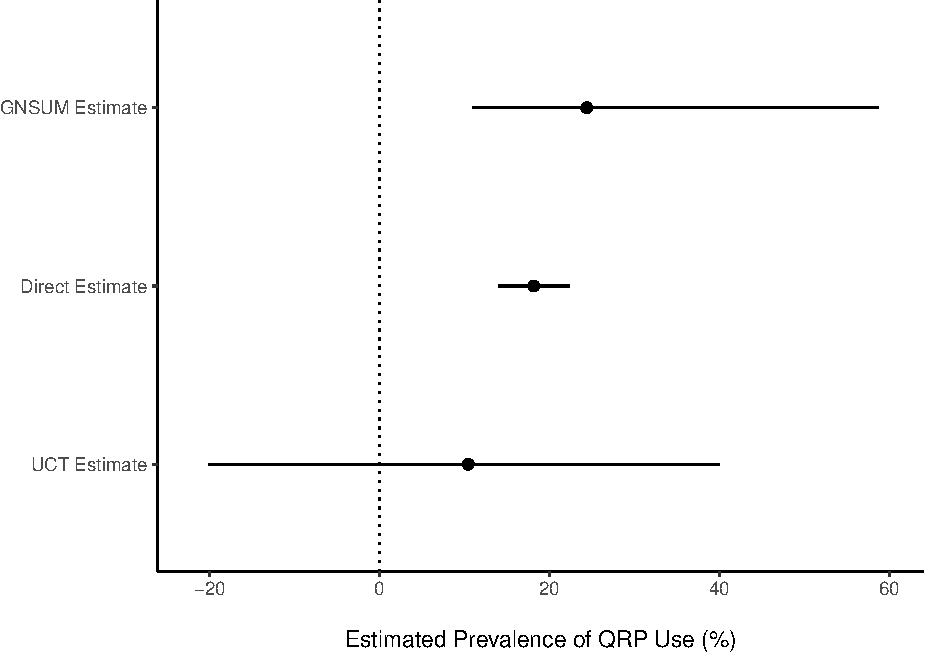
\includegraphics{papaja_test_files/figure-latex/fig1-1.pdf}
\caption{\label{fig:fig1}\label{fig:fig1}Estimates of the current prevalence
of users of questionable research practices using three different
estimators; the Generalized Network Scale-Up Method (GNSUM), the Direct
Estimate, and the Unmatched Count Technique (UCT). Point estimates with
95\% bootstrapped confidence intervals.}
\end{figure}

\subsection{Direct Estimate}\label{direct-estimate-1}

To ensure the highest number of participants in our game of contacts,
half of the total population were asked to participate in Survey 3,
which contained our direct estimate question. Thus, psychologists were
solicited, and we received responses to Survey 3 able to be analyzed. Of
the participants, indicated they had used at least one QRP in the past
12 months. Using Equation 1, we calculated QRP prevalence to be 18.18\%
(bootstrapped 95\% confidence interval {[}13.96\%, 22.40\%{]}). This
corresponds to an estimated 1291 American psychologists currently using
QRPs.

It is possible this estimate is underestimating the true number of
psychologists using QRPs. For one, social desirability may influence QRP
users to conceal their identity when asked directly. In that case, our
estimate is only generated by those participants willing to reveal their
identity. Given the somewhat critical social environment for QRP users
(Fiske, 2016), it is reasonable to believe some participants withheld
their identity when we asked directly. The following indirect estimation
methods sought to mitigate this social desirability bias.

\subsection{Unmatched Count
Technique}\label{unmatched-count-technique-1}

The remaining psychologists contacted were asked to participate in our
unmatched count estimate with randomized into the innocuous list
condition, and randomized into the sensitive list condition.

The average number of list items corresponding to participants in the
innocuous list condition was . The average number of list items
corresponding to participants in the sensitive list condition was .
Using Equation 2, we calculated QRP user prevalence to be 10.46\%
{[}-20.19\%, 22.40\%{]}. This corresponds to an estimated 743 American
psychologists currently using QRPs.

It was unexpected that an UCT estimate lower than our direct estimate
would be calculated. Typically, due to reducing response bias, UCT
estimates tend to be larger than direct estimates when the behavior or
identity in question is stigmatized ({\textbf{???}}; Gervais \& Najle,
2017; Wolter \& Laier, 2014). The fact that the bootstrapped confidence
interval crosses zero indicates instibility in the sensitive list being
consistantly larger than the control list. It is likely our relatively
low number of participants in our UCT estimate () led this calculation
to be overly sensitive to individual responses. This is not the first
time the UCT has provided smaller estimates than a direct estimate
({\textbf{???}}), though given the high variability, we do not have
confidence that this UCT estimate is a valid estimate of current QRP
use.

\subsection{Generalized Network Scale-Up
Estimate}\label{generalized-network-scale-up-estimate}

All participants who were randomized into the UCT estimate were also
asked to answer questions about their social networks, and to estimate
how many researchers they know who have used at least one QRP in the
past 12 months. Participants who were randomized into the direct
estimate and who self-identified as a QRP user in that estimate were
also asked to answer questions about their social network and to
participate in the game of contacts method. Participants in the direct
estimate who did not self-identify as a QRP user were asked questions
about their social network as well, but were not asked how many
researchers they know who have used at least one QRP in the past 12
months. Therefore, we collected social network responses from
participants from the general frame population (to be used in estimating
\(\delta\)), responses from participants who self-identified as QRP
users who also completed the game of contacts (to be used in estimating
\(\tau\)), and responses from participants who estimated the number of
researchers they know who have used at least one QRP in the past 12
months.

These identified QRP users, and know a collective researchers. Given the
total frame population is 7101, we are fairly confident all members were
identified at least once by our participants. Using the network scale-up
in Equation 3, this generates an estimate of 1.42\% {[}0.85\%,
2.14\%{]}. This estimate serves as the base starting point for Equation
4, the Generalized Network Scale-Up Estimator, detailed below.

Equation 4 relaxes the assumptions of equal network size and total
information transmission by incorporating \(\tau\) and \(\delta\). Using
the responses from the general population, plus the responses from the
participants who indicated using a QRP in the past 12 months, we
estimate \(\delta\) as 0.97. Using the game of contacts, we estimate
\(\tau\) as 0.06. Using Equation 4, we estimate QRP user prevalence to
be 24.40\% {[}10.93\%, 58.74\%{]}. This corresponds to an estimated 1733
American psychologists currently using QRPs.

To assess the accuracy of participants in estimating the size of this
unknown group (QRP users), we asked questions about 24 populations of
known size (number of researchers named David, named Janet, etc). The 24
names were gender balanced and represented common, uncommon, and rare
names that exist within the census of the frame population. The size
estimates of these populations of known size can be seen in Figure
\ref{fig:fig2}. These estimates seem reasonable and closely mirror the
actual prevalence of these groups. The fact that the same estimator in
the same group of participants can generate reasonable estimates for
populations of known size is encouraging evidence of the accuracy of our
estimate of the number of recent QRP users utilizing the generalized
network scale-up estimate.

\begin{figure}
\centering
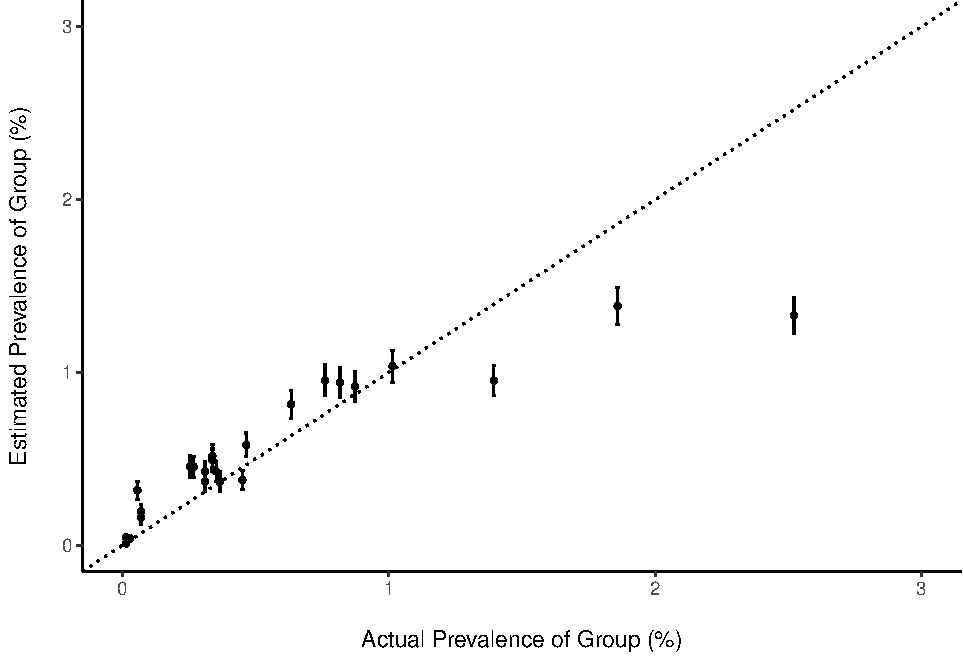
\includegraphics{papaja_test_files/figure-latex/fig2-1.pdf}
\caption{\label{fig:fig2}\label{fig:fig2}Validation of Network Scale-Up
Estimates using 24 groups of known size. Each point represents one
group, with 95\% confidence intervals. Dotted line represents when
estimated group size equals actual group size.}
\end{figure}

\section{DISCUSSION}\label{discussion}

To the best of our knowledge, this is the first report of the prevalence
of QRPs in a proximal timespan. As such, it is difficult to draw
conclusions about the magnitude of our estimates when compared to
previous estimates. Compared to John, Loewenstein, and Prelec (2012) and
Agnoli, Wicherts, Veldkamp, Albiero, and Cubelli (2017), we estimate
lower rates of questionable research practices. Compared to Fiedler and
Schwarz (2016), however, we estimate higher rates of these practices.
Our definition of \enquote{questionable research practices} were the
same ones used in John et al. (2012) and Agnoli et al. (2017), but was
restricted to a timespan of only 15 months, so it is reasonable that our
estimates would be lower than those with an unrestricted time of QRP
use. Since we used those same QRP definitions, is also reasonable that
our estimates would be higher than those described by Fiedler and
Schwarz (2016), who changed the definition of each QRP. We also measured
true \enquote{prevalence}, that is, the commonality of a behavior within
a designated time frame, which was a point of difference between John et
al. (2012) and Fiedler and Schwarz (2016).

This is also the first report to use the network scale-up and
generalized network-scale up estimators to investigate the ongoing
reproducibility issues in psychology. Re-framing QRP prevalence away
from the individual behavior and towards the user state brings our
field-wide problems more into scope with existing literature on stigma
and concealable identities. For example, much work has been done
focusing on how increasing stigma inadvertently locks individuals into
detrimental behaviors (Stuber2009), and how revealing a concealed
identity can increase well-being by reducing the stress of being exposed
(Chaudoir \& Quinn, 2010). Framing QRP use in terms of the individual
may help the field reduce QRP use by increasing awareness of the effects
of stigma and support.

\subsection{Implications}\label{implications}

These estimates serve as a baseline to measure the effectiveness of
current initiatives, as well as a foundation for new ones. While much
work is being done to grow support for interventions such as
pre-registration (CITATION) and Registered Reports (CITATION), it is
currently unknown what quantitative effect these are having on curbing
behaviors associated with inflated Type I error such as QRPs. By
performing follow-up estimates, the field can use these baseline
estimates to measure the effectiveness of these programs and make
informed decisions on their effectiveness.

\subsection{Limitations \& Future
Directions}\label{limitations-future-directions}

Our unmatched count estimate produced a value with a confidence interval
that crossed zero, meaning there was sufficient variance to destabilize
the group difference we observed. As mentioned previously, the
relatively low number of participants for the unmatched count estimate
() contributed to this high variability. Future work using the unmatched
count technique would benefit from larger sample sizes (as demonstrated
in Gervais and Najle (2017), which used 2000 participants).

These estimates were limited to American psychologists, though we know
that these issues are not contained solely in the United States (Stapel
CITATION). Future studies estimating the prevalence of QRPs in other
countries will be an important next step. Some of this work has already
started through the Horizon 2020 framework in the European Union
(PRINTEGER CITATION), though more innovative work will be required to
better understand the scope of the problems faced by our field.

\subsection{Conclusion}\label{conclusion}

By directly asking participants about their use of QRPs, we estimate
18.18\% have used at least one QRP in the past 12 months, and the
generalized network scale up estimate is 24.40\%, which corresponds to
between 1291 and 101 American psychologists. While some argue the
narrative of the \enquote{replication crisis} is overblown (Fanelli,
2018), the current work illustrates how common these behaviors that
inflate false-positive findingss are. Although many have called for
changes in statistical inference practices to mitigate false-positive
findings {[}Lakens et al. (2018); Benjamin2017{]}, it is important that
we as a field continue to focus on disincentivizing the use of
questionable research practices (and other behavioral degrees of
freedom) among our peers and coworkers for the betterment of our
science.

\newpage

\section{References}\label{references}

\begingroup
\setlength{\parindent}{-0.5in} \setlength{\leftskip}{0.5in}

\hypertarget{refs}{}
\hypertarget{ref-Agnoli2017}{}
Agnoli, F., Wicherts, J. M., Veldkamp, C. L. S., Albiero, P., \&
Cubelli, R. (2017). Questionable research practices among Italian
research psychologists. \emph{PLoS ONE}, \emph{12}(3), 1--17.
doi:\href{https://doi.org/10.1371/journal.pone.0172792}{10.1371/journal.pone.0172792}

\hypertarget{ref-Ahrnsbrak2017}{}
Ahrnsbrak, R., Bose, J., Hedden, S., Lipari, R., \& Park-Lee, E. (2017).
Key Substance Use and Mental Health Indicators in the United States:
Results from the 2016 National Survey on Drug Use and Health.
\emph{Substance Abuse and Mental Health Services Administration},
\emph{7}(1), 877--726.
doi:\href{https://doi.org/10.1016/j.drugalcdep.2016.10.042}{10.1016/j.drugalcdep.2016.10.042}

\hypertarget{ref-Bernard2010}{}
Bernard, H. R., Hallett, T., Iovita, A., Johnsen, E. C., Lyerla, R.,
McCarty, C., \ldots{} Stroup, D. F. (2010). Counting hard-to-count
populations: the network scale-up method for public health.
\emph{Sexually Transmitted Infections}, \emph{86 Suppl 2}, ii11--5.
doi:\href{https://doi.org/10.1136/sti.2010.044446}{10.1136/sti.2010.044446}

\hypertarget{ref-Chaudoir2010}{}
Chaudoir, S. R., \& Quinn, D. M. (2010). Revealing Concealable
Stigmatized Identities: The Impact of Disclosure Motivations and
Positive First-Disclosure Experiences on Fear of Disclosure and
Well-Being. \emph{Journal of Social Issues}, \emph{66}(3), 570--584.
doi:\href{https://doi.org/10.1111/j.1540-4560.2010.01663.x}{10.1111/j.1540-4560.2010.01663.x}

\hypertarget{ref-Connelly1995}{}
Connelly, N. A., \& Brown, T. L. (1995). Use of Angler Diaries to
Examine Biases Associated with 12-Month Recall on Mail Questionnaires.
\emph{Transactions of the American Fisheries Society}, \emph{124}(3),
413--422.
doi:\href{https://doi.org/10.1577/1548-8659(1995)124\%3C0413:uoadte\%3E2.3.co;2}{10.1577/1548-8659(1995)124\textless{}0413:uoadte\textgreater{}2.3.co;2}

\hypertarget{ref-Fanelli2018}{}
Fanelli, D. (2018). Is science really facing a reproducibility crisis,
and do we need it to? \emph{Proceedings of the National Academy of
Sciences of the United States of America2}, \emph{in press}, 1--4.
doi:\href{https://doi.org/10.1073/pnas.1708272114}{10.1073/pnas.1708272114}

\hypertarget{ref-Fiedler2016}{}
Fiedler, K., \& Schwarz, N. (2016). Questionable Research Practices
Revisited. \emph{Social Psychological and Personality Science},
\emph{7}(1), 45--52.
doi:\href{https://doi.org/10.1177/1948550615612150}{10.1177/1948550615612150}

\hypertarget{ref-Fiske2016}{}
Fiske, S. T. (2016). Mob Rule or Wisdom of Crowds. \emph{APS Observer}.

\hypertarget{ref-Gervais2017}{}
Gervais, W. M., \& Najle, M. B. (2017). How many atheists are there?
\emph{Social Psychological and Personality Science}, 1948550617707015.

\hypertarget{ref-John2012}{}
John, L. K., Loewenstein, G., \& Prelec, D. (2012). Measuring the
Prevalence of Questionable Research Practices With Incentives for Truth
Telling. \emph{Psychological Science}, \emph{23}(5), 524--532.
doi:\href{https://doi.org/10.1177/0956797611430953}{10.1177/0956797611430953}

\hypertarget{ref-Lakensabc1860}{}
Lakens, D., Adolfi, F. G., Albers, C. J., Anvari, F., J Apps, M. A.,
Argamon, S. E., \ldots{} Lino de Oliveira, C. (2018). Justify Your
Alpha: A Response to `` Redefine Statistical Significance''.
\emph{Nature Human Behavior}, \emph{2}, 168--171.

\hypertarget{ref-Landen1995}{}
Landen, D. D., \& Hendricks, S. (1995). Effect of recall on reporting of
at-work injuries. \emph{Public Health Reports (Washington, D.C. :
1974)}, \emph{110}(3), 350--4.
doi:\href{https://doi.org/10.1016/s0022-4375(97)90342-x}{10.1016/s0022-4375(97)90342-x}

\hypertarget{ref-Salganik2011}{}
Salganik, M. J., Fazito, D., Bertoni, N., Abdo, A. H., Mello, M. B., \&
Bastos, F. I. (2011). Assessing network scale-up estimates for groups
most at risk of HIV/AIDS: Evidence from a multiple-method study of heavy
drug users in Curitiba, Brazil. \emph{American Journal of Epidemiology},
\emph{174}(10), 1190--1196.
doi:\href{https://doi.org/10.1093/aje/kwr246}{10.1093/aje/kwr246}

\hypertarget{ref-Salganik2012b}{}
Salganik, M. J., Mello, M. B., Abdo, A. H., Bertoni, N., Fazito, D., \&
Bastos, F. I. (2012). The Game of Contacts: Estimating the Social
Visibility of Groups. \emph{Networks}, \emph{33}(1), 70--78.
doi:\href{https://doi.org/10.1016/j.socnet.2010.10.006.The}{10.1016/j.socnet.2010.10.006.The}

\hypertarget{ref-Salganik2012}{}
Salganik, M. J., Mello, M., Abdo, A., Bertoni, N., Fazito, D., \&
Bastos, F. (2012). The Game of Contacts: Estimating the Social
Visibility of Groups, \emph{100}(2), 130--134.
doi:\href{https://doi.org/10.1016/j.pestbp.2011.02.012.Investigations}{10.1016/j.pestbp.2011.02.012.Investigations}

\hypertarget{ref-NHIS2006}{}
United States Census Bureau. (2018). \emph{National health Interview
Survey: CAPI Manual for NHIS Field Representative} (No. January).
Retrieved from
\href{ftp://ftp.cdc.gov/pub/health\%7B/_\%7Dstatistics/nchs/Survey\%7B/_\%7DQuestionnaires/NHIS/2006/frmanual.pdf}{ftp://ftp.cdc.gov/pub/health\{\textbackslash{}\_\}statistics/nchs/Survey\{\textbackslash{}\_\}Questionnaires/NHIS/2006/frmanual.pdf}

\hypertarget{ref-Wolter2014}{}
Wolter, F., \& Laier, B. (2014). The Effectiveness of the Item Count
Technique in Eliciting Valid Answers to Sensitive Questions. An
Evaluation in the Context of Self-Reported Delinquency. \emph{Survey
Research Methods}, \emph{8}(3), 153--168.

\endgroup






\end{document}
